\section{Transportschicht}

\paragraph{Ziele und Prinzipien}
\begin{itemize}
	\item Kommunikation zwischen Prozessen
  \item \emph{Verbergen von Transportdetails vor höheren Schichten}
  \item \emph{Bereitstellung von Transportdiensten}
  \begin{itemize}
    \item[\( \leadsto \)] logische \textbf{Nutzer-zu-Nutzer-Kommunikation} (Anwendungen)
    \item Vermittlungsschicht: Ende-zu-Ende-Kommunikation (Endsysteme)
  \end{itemize}
  \item Transportprotokoll läuft auf Endsystemen
  \item \textbf{Sender}:
  \begin{itemize}
    \item \emph{Segmentieren} von Anwendungsnachrichten
    \item \emph{Weiterleiten} an Vermittlungsschicht
  \end{itemize}
  \item \textbf{Empfänger}:
  \begin{itemize}
    \item \emph{Reassemblieren} der Segmente in Nachrichten
    \item \emph{Weiterleiten} an Anwendungsschicht
  \end{itemize}
\end{itemize}

\paragraph{Protokolle}
\begin{itemize}
  \item \textbf{UDP} (\emph{user datagram protocol}): verbindungsloser, \emph{unzuverlässiger} Transport
  \item \textbf{TCP} (\emph{transmission control protocol}): verb.-orientierter, \emph{zuverlässiger} Transport
  \item \textbf{Unzuverlässig}: keine Fehlermaßnahmen; unklar, ob Daten korr. ankommen
  \item \textbf{Zuverlässig}: Fehlermaßnahmen garantieren
  \begin{itemize}
    \item \emph{Korrektheit}, \emph{Vollständigkeit}, \emph{Reihenfolge}
    \item keine \emph{Duplikate}, keine \emph{Phantom-Pakete}
  \end{itemize}
\end{itemize}

\paragraph{(De-)Multiplexing --- Ports}
\begin{itemize}
\item Ausliefern von Segmenten an den korrekten Socket (nutze Transportheader)
  \item Port = \emph{Adresse der Transportschicht} (Kennzeichnung der Prozesse)
  \item Unstrukturierte Nummer (16 Bit), 0 bis 65535
  \item \textbf{Well known ports}: viele Portnummern unter 1024 für häufig benutzte Anwendungen reserviert (Telnet, HTTP, SMTP, FTP, \dots)
  \item Eindeutige Adressierung eines Prozesses: ``IP-Adresse:Port''
\end{itemize}

\paragraph{UDP (User Datagram Protocol)}
\begin{itemize}
  \item \emph{Sehr einfaches Transportprotokoll mit sehr geringem Overhead (8 Byte)}
  \item \textbf{Eigenschaften}:
  \begin{itemize}
    \item (De-) Multiplexen von Segmenten für Prozesse
    \item \emph{Prüfsumme} für Bitfehler
    \item \emph{best effort}: keine Zusagen über Auslieferung bei Empfänger
    \item \emph{verbindungslos}
    \item \emph{keine Verbindungsaufbauphase}: sofortiges Senden \( \leadsto \) keine Verzögerung
    \item \emph{kein Verbindungszustand}: keine Verbindungsinformationen im Endsystem \( \leadsto \) skaliert z.B. für Server besser
    \item \emph{Unreguliertes Senden}: kann Daten so schnell senden wie von Anwendung geliefert und von Netz abgenommen
  \end{itemize}
  \item \textbf{Verwendung}: \textbf{DNS}, Multimedia (VoIP)
\end{itemize}
\begin{figure}[H]\centering\label{UDPAufbau}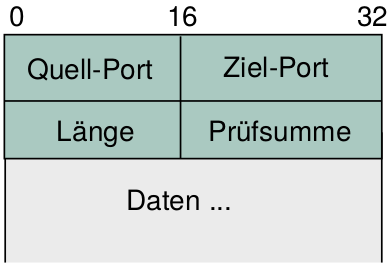
\includegraphics[width=0.3\linewidth]{UDPAufbau}\end{figure}

\paragraph{Bitfehler}
\begin{itemize}
  \item \emph{Verfälschung von Bits während dem Datentransport}
  \item \textbf{Ursachen}: Dämpfung, Übersprechen, Synchronisationsverlust, \dots
  \item \textbf{Einzelbitfehler}: ein \emph{einzelnes} Bit fehlerhaft
  \item \textbf{Bündelfehler}: mehrere direkt aufeinanderfolgende Bits fehlerhaft
    \item \textbf{Bitfehlerrate}: Maß für Fehlerhäufigkeit \( = \tfrac{\text{Summe gestörter Bits}}{\text{Summe übertragener Bits}} \)
\end{itemize}

\paragraph{Bitfehler --- Erkennung/Korrektur}
\newcommand{\dmin}{\ensuremath{d_{\min}}}
\begin{itemize}
	\item \textbf{Fehlererkennung} (\emph{error detecting code}, EDC)
	\item \textbf{Fehlerkorrektur} (\emph{forward error correction}, FEC)
	\item Hinzufügen von Redundanz (Paritätsbit (\( \dmin = 2 \)), Prüfsumme, \dots) \\*
		\( \leadsto \) Ausreichend stark unterscheidende Codewörter 
	\item \textbf{Hamming-Abstand} \( d_{i,j} \): \#Stellen, an denen sich Codewörter unterscheiden
	\item Hamming-Abstand des Codes \( \dmin \): Min Abstand zw Codewörtern
	\item Erkennen von bis zu \( \dmin - 1 \) Bitfehlern
	\item Korrigieren von bis zu \( \lfloor \frac{\dmin - 1}{2} \rfloor \) Bitfehlern
	\item Kontrollmatrix \( H \), für übertragenes Wort \( w \) gilt:
	\begin{itemize}
    \item Syndrom \( S = w \cdot H^T = 0 \), falls Übertragung fehlerfrei (\( w \) ist Codewort)
    \item Ansonsten kann das Syndrom die Position des Bitfehlers angeben
  \end{itemize}
\end{itemize}

\paragraph{Bitfehler --- Internet-Prüfsumme (UDP, TCP, IP)}
\begin{itemize}
  \item \textbf{Prinzip}: Aufaddieren aller übertragenen Wörter (16 Bit, als Integer interpretiert), evtl. Übertrag addieren, bitweise negieren (Einerkomplement)
  \item \textbf{Nachteil}: Falsche Reihenfolge kann nicht erkannt werden
\end{itemize}
\begin{figure}[H]\centering\label{Internetpruefsumme}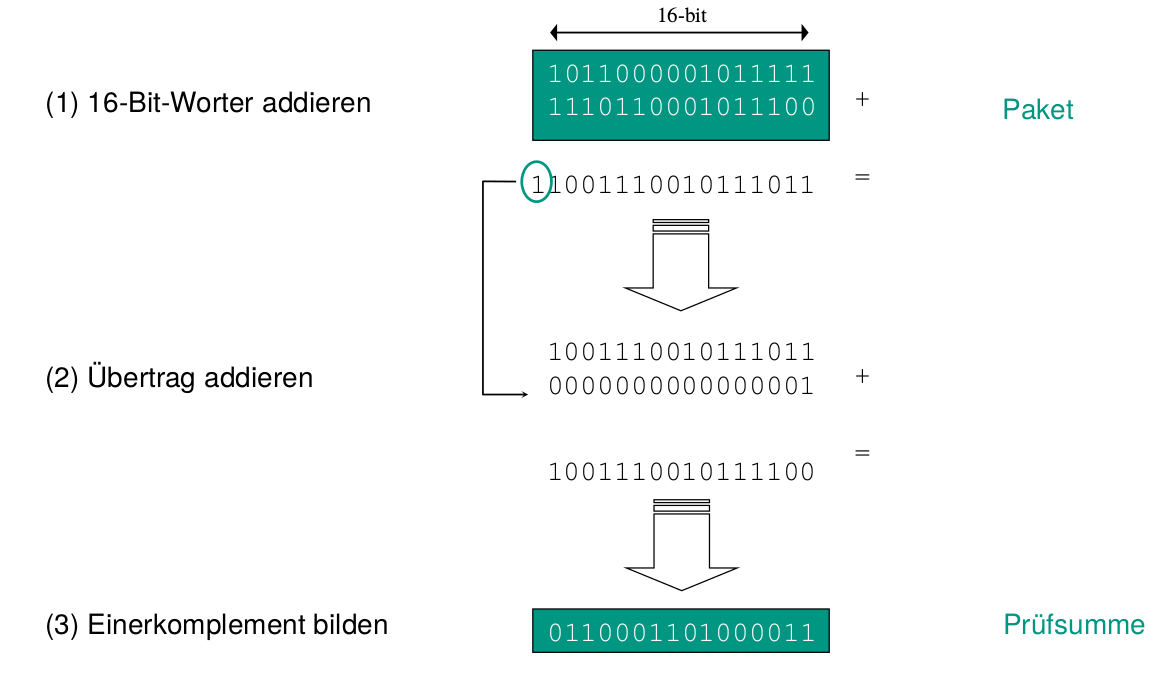
\includegraphics[width=0.33\textwidth]{Internetpruefsumme}\end{figure}

\paragraph{Paketfehler}
\begin{itemize}
	\item \emph{Verlust / Duplizierung von Paketen}
	\item \emph{Phantom-Pakete}
	\item \emph{Reihenfolgenvertauschung}
	\item \textbf{Ursachen}: Zwischensystemüberlastung, Unterschiedliche Wege durch Netz, Verfrühte Datenwiederholung, \dots
\end{itemize}

\paragraph{Paketfehler --- Erkennung/Korrektur}
\begin{itemize}
  \item \textbf{Sequenznummern} (\emph{sequence number}):
  \begin{itemize}
    \item Pakete werden durchnummeriert
    \item Empfänger kann Vollständigkeit, Reihenfolge, Duplikate feststellen
  \end{itemize}
  \item \textbf{Quittungen} (\emph{acknowledgements}): Empfänger informiert Sender, ob Paket angekommen ist
  \begin{itemize}
    \item \emph{positiv}: Daten erhalten (ACK)
    \item \emph{negativ}: Daten \emph{nicht} erhalten (NACK)
    \item \emph{selektiv}: Einzelnes Paket
    \item \emph{kumulativ}: Paketmenge (bis zu einer Sequenznummer)
  \end{itemize}
  \item \textbf{Zeitgeber} (\emph{timer}):
  \begin{itemize}
    \item Sender merkt nicht, wenn ein Paket nicht angekommen ist
    \item Nach zeitl Obergrenze wird \emph{vermutet}, dass Paket nicht angekommen ist \\* \( \leadsto \) \emph{Sendewiederholung} (\emph{retransmissions})
  \end{itemize}
  \item \textbf{Automatic Repeat Request (ARQ)}: Sendewiederholungsvariante: Sender erhält positive Quittungen, kann Sendewiederholungen ausführen
\end{itemize}

\paragraph{ARQ --- Stop-and-Wait}
\begin{itemize}
  \item \textbf{Prinzip}: Sender wartet auf Quittung nach jedem gesendeten Paket
  \begin{itemize}
    \item Erst \emph{nach} Quittungserhalt wird nächstes Paket gesendet
    \item Keine Quittung nach Wartezeit (Zeitgeber) \( \leadsto \) Sendewiederholung
  \end{itemize}
  \item \textbf{Sequenznummern}: 1 Bit (Empfänger kann nur Paket doppelt erhalten)
  \item Sehr einfaches ARQ-Verfahren (z.B. im WLAN)
  \item \textbf{Auslastung}: \( U = \tfrac{1}{1+2a} \) (mit \( a = \tfrac{t_a}{t_s} \)), \( t_{Ges} = t_s + 2t_a \)
  \item $\textbf{a} = \tfrac{t_a}{t_s}$ ist Verhältnis der Länge des Mediums in Bit zur Länge der Dateneinheit
  \item Bandbreitenverzögerungsprodukt \( \tfrac{m}{v}r \): Länge des Mediums in Bit \\*
  (Länge \( m \), Ausbreitungsgeschwindigkeit \( v \), Datenrate \( r \))
\end{itemize}

\paragraph{ARQ --- Go-Back-N}
\begin{itemize}
  \item \textbf{Zeil}: Leistungsfähigkeit im Vergleich zu Stop-and-Wait erhöhen
  \item \textbf{Prinzip}: Sender sendet mehrere Pakete bis Quittungspflicht
  \begin{itemize}
    \item Begrenzte Anzahl (\textbf{Fenster}, \emph{window}) an nicht quittierten Paketen
    \item Quittierung durch kumulative Quittungen
  \end{itemize}
  \item \textbf{Fehlerfall}:
  \begin{itemize}
    \item Empfänger empfängt fehlerhaftes Paket, verwirft alle nachfolgenden Pakete
    \item Sender wiederholt bei Ablauf des Zeitgebers alle nicht quittierten Pakete
  \end{itemize}
  \item \textbf{Auslastung}: \( U = \begin{cases}
    1 & W \geq 1+2a \\
    \tfrac{W}{1+2a} & \text{sonst}
  \end{cases} \)
\end{itemize}

\paragraph{ARQ --- Selective Repeat}
\begin{itemize}
  \item \textbf{Ziel}: Datenaufkommen von Go-Back-N reduzieren
  \item \textbf{Prinzip}: Wie Go-Back-N, Empfänger quittiert selektiv
  \item \textbf{Fehlerfall}: Empfänger puffert und bestätigt nachfolgende, korrekte Pakete \( \leadsto \) Sender wiederholt nur nicht korrekt empfangene Pakete
  \item \textbf{Selective Repeat}: Fehler-Paket bleibt unbestätigt, Sender wartet auf Timeout
  \item \textbf{Selective Reject}: Empfänger sendet für Fehler-Paket negative Quittung \\* \( \leadsto \) Sender wiederholt sofort und wartet nicht auf Timeout
\end{itemize}

\paragraph{Paketfehler --- Vorwärtsfehlerkorrektur}
\begin{itemize}
  \item \textbf{Ziel}: Empfänger muss nur drei von vier Paketen korrekt empfangen um fehlendes Paket rekonstruieren zu können
  \item \textbf{Prinzip}: XOR-Verknüpfung der drei Pakete \( \leadsto \) fehlendes Paket
\end{itemize}

\paragraph{Flusskontrolle}
\begin{itemize}
  \item \textbf{Problem}: \emph{Überlastung} von Empfänger durch Sender \( \leadsto \) Datenverlust
   \item Sender muss Größe des Empfangspuffers berücksichtigen
  \item \textbf{Anforderungen}: einfach, fair, stabil, möglichst wenig Netzressourcen nutzen
\end{itemize}

\paragraph{Flusskontrolle --- Halt-und-Weiter}
\begin{itemize}
  \item \textbf{Prinzip}: Empfänger sendet \code{halt} und \code{weiter}-Signal
  \item \textbf{Bewertung}:
  \begin{itemize}
    \item nur auf Vollduplex verwendbar
    \item nicht effektiv bei hohen Verzögerungen
    \item Probleme bei Verlust der \code{halt}-Meldung
  \end{itemize}
  \item \textbf{Beispiel}: Fast-/Gigabit-Ethernet
\end{itemize}

\paragraph{Flusskontrolle --- Stop-and-Wait}
\begin{itemize}
  \item \textbf{Prinzip}: Empfänger sendet Quittung erst, wenn er wieder empfangen kann
   \item Sender wird durch Zurückhalten gebremst
  \item \textbf{Problem}: Sender kann nicht zwischen Datenverlust und Überlastung unterscheiden
\end{itemize}

\paragraph{Flusskontrolle --- Kreditbasiert}
\begin{itemize}
  \item \textbf{Prinzip}:
  \begin{itemize}
    \item Sender kann höchstens \( n \) Pakete unquittiert senden
    \item \( n \) = Pufferkapazität des Senders \( \Rightarrow \) \textbf{Sendekredit}
    \item Alternativbezeichnung: Fenster (\emph{sliding window})
    \item Fenster wird durch korrekte positive Quittung weitergeschaltet
    \item Empfänger kann Kredit bestimmen (z.B. in TCP)
  \end{itemize}
\end{itemize}

\paragraph{TCP --- Prinzip}
\begin{itemize}
	\item \textbf{Zuverlässiger}, verbindungsorientierter Transportdienst zwischen Anwendungen
  \item \emph{Erhält Bytestrom von Anwendung (über Socket), übergibt TCP-Segmente an IP}
  \item Wann wird ein TCP-Segment erzeugt und versendet?
  \begin{itemize}
    \item MSS (\emph{maximum segment size}): Anwendungsdatenlänge (z.B. 1460 Byte)
    \item Push (\code{PSH} in TCP-Segmentkopf): Sender verlangt sofortiges Senden
    \item Zeitgeber: Nach Zeitintervall der Inaktivität vorhandene Daten senden
  \end{itemize}
  \item \textbf{Fehlerkontrolle}: Sequenznr., Prüfsumme, Quittierungen, Sendewdh-en
  \item \textbf{Sequenznummern}: pro Byte, nicht pro Segment (erstes Byte in Segment, initiale Sequenznummer von Endsystem \emph{zufällig} gewählt)
  \item \textbf{Quittungen: } positive kumulative Quittungen (Sequenznummer des \emph{nächsten} Bytes, das erwartet wird), mit Datensegment versendet (\emph{piggybacked} im Header)
\end{itemize}
\begin{figure}[H]\centering\label{TCPAufbau}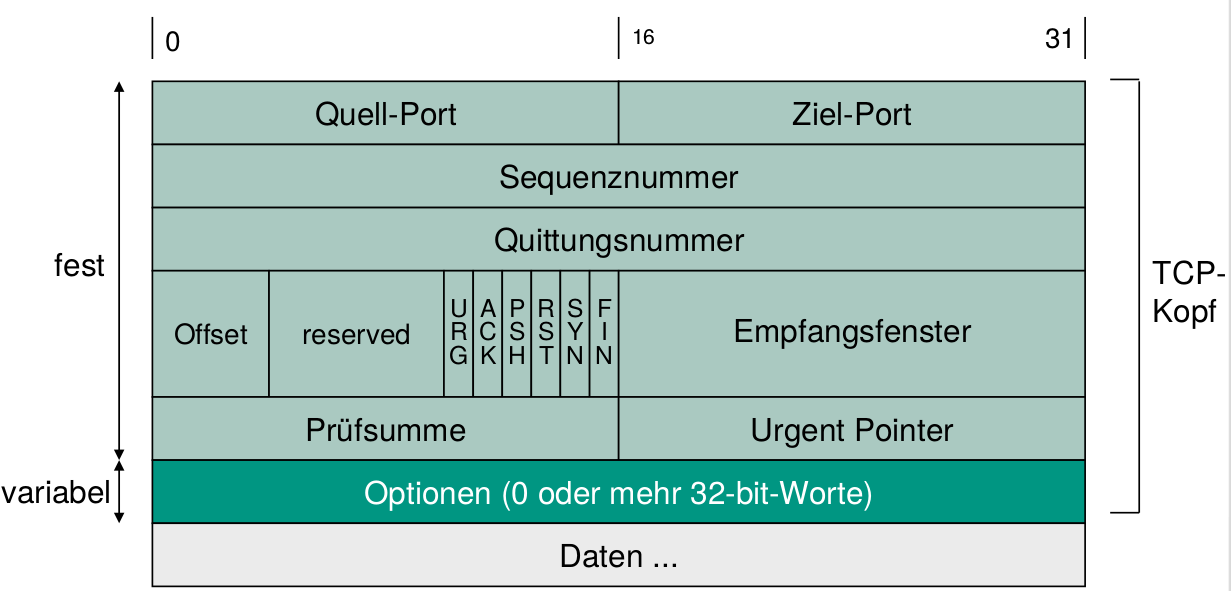
\includegraphics[width=0.33\textwidth]{TCPAufbau}\end{figure}

\paragraph{TCP --- Felder}
\begin{itemize}
  \item \textbf{Quell-/Ziel-Port}: Identifizieren Verbindungsendpunkte
  \item \textbf{Sequenznummer}: gemessen in Byte, nicht pro Segment
  \item \textbf{Quittung}: nächste von Empfänger erwartete Sequenznummer
  \item \textbf{Offset}: Anzahl 32 Bit-Wörter in TCP-Kopf
  \item \textbf{URG}: 1, falls \emph{urgent pointer} verwendet wird (idR leer)
  \item \textbf{SYN}: Bei Verbindungsaufbau \emph{connection request} oder \emph{connection confirmation}
  \item \textbf{ACK}: Gültigkeit des Quittungsfeldes; unterscheidet bei gesetztem SYN-Bit zwischen Request und Confirmation; 
  \item \textbf{FIN}: Sender möchte nichts mehr senden
  \item \textbf{RST}: Verbindung zurücksetzen
  \item \textbf{PSH}: übergebene Daten sollen sofort weitergeleitet werden (idR leer)
  \item \textbf{Empfangsfenster}: Flusskontrolle
  \item \textbf{Prüfsumme}: Prüfsumme über TCP-Kopf, Daten und Pseudoheader
  \item \textbf{Urgent-Zeiger}: relativer Zeiger auf wichtige Daten
  \item \textbf{Optionen-Feld}: Optionen variabler Länge (\( n * 32 \) Bit)
\end{itemize}

\paragraph{TCP --- Flusskontrolle}
\begin{itemize}
  \item \textbf{Ziel}: Empfänger nicht überlasten
  \item \textbf{Prinzip}: Empfänger reserviert Puffer pro Verbindung (expl Kreditvergabe)
  \begin{itemize}
    \item \code{RcvBuffer}: gesamter Pufferplatz (default 4096 Byte)
    \item \code{RcvWindow}: freier Pufferplatz (Empfangsfenster) in TCP-Header mitsenden
    \item Sender sendet nicht mehr unbestätigt als in \code{RcvWindow} passt
  \end{itemize}
\end{itemize}
\begin{figure}[H]\centering\label{TCPBuffer}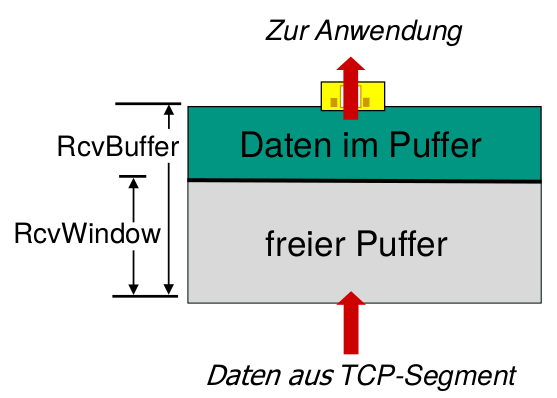
\includegraphics[width=0.2\textwidth]{TCPBuffer}\end{figure}

\paragraph{TCP --- Verbindungen}
\begin{itemize}
  \item \textbf{Verbindungslos (UDP)}: Daten werden ohne vorherigen Handshake gesendet
  \begin{itemize}
    \item \emph{Vorteil}: schnelle Datenversendung möglich
    \item \emph{Nachteil}: kein Feedback, keine Bestätigung
  \end{itemize}
  \item \textbf{Verbindungsorientiert (TCP)}: Expliziter Verbindungsaufbau/-abbau
  \begin{itemize}
    \item \emph{Vorteil}: Kommunikationsparameter können ausgehandelt werden
    \item \emph{Nachteile}: Verzögerter Datenaustausch, Overhead ggf größer als Daten
  \end{itemize}
  \item Probleme mit 2-Wege-Handshake: Verzögerungen + Wiederholte Nachrichten können zu halboffenen Verbindungen führen
  \item \textbf{3Way-Handshake}: SYN, SYN/ACK, ACK (letztes ACK kann Nutzdaten enth)
  \item \textbf{Abbau}: Richtungen unabhängig jeweils durch FIN, ACK schließen, danach Warten vor vollständigem löschen (falls Wiederholungen auftreten)
  \item \textbf{Abbruch}: RST, Verbindung wird unmittelbar geschlossen
\end{itemize}

\paragraph{TCP --- Staukontrolle}
\begin{itemize}
	  \item \textbf{Ziel}: Netz nicht überlasten (Pufferüberläufe in Routern vermeiden)
	\item \textbf{Staukontrollfenster} (\emph{congestion window}, \code{CWnd}) beschränkt maximale Datenmenge: \( \text{LastByteSent} - \text{LastByteAcked} \leq \text{min} \{ \text{CWnd}, \text{RcvWindow} \} \)
	\item \textbf{Stauerkennung}: Vermutung einer Stausituation bei ausbleibender Quittung
	\item \textbf{Staubehebung}: Reduktion von \code{CWnd}
	\item Langsames Erhöhen von \code{CWnd} \( \leadsto \) herantasten an Netzkapazität
  \item \textbf{Start}: \code{CWnd} = 1 \code{MSS} (\emph{maximum segment size})
  \item \textbf{Slow-Start}, falls \code{CWnd} \( \leq \) \code{SSTresh} \& Quittungen rechtzeitig da \\* \( \leadsto \) \emph{exponentielles} Erhöhen \code{CWnd} (\code{CWnd} += 1 bei jeder empfangenen Quittung)
  \item \textbf{Congestion Avoidance}, falls \code{CWnd} > \code{SSTresh} \& Quittungen rechtzeitig da \\* \( \leadsto \) \emph{lineares} Erhöhen \code{CWnd} (\code{CWnd} += \( \tfrac{1}{\text{\code{CWnd}}} \) bei jeder empfangenen Quittung)
  \item \textbf{Congestion}, falls Quittung nicht rechtzeitig da: Stau vermutet
  \begin{itemize}
    \item \( \text{\code{SSTresh}} = \text{max}(\tfrac{\text{FlightSize}}{2}, 2*\text{MSS}) \) (FlightSize = unquittierte ges Daten)
    \item \code{CWnd} zurücksetzen (neue Slow-Start-Phase): \code{CWnd} = 1 \code{MSS}
  \end{itemize}
\end{itemize}
\begin{figure}[H]\centering\label{TCPStaukontrolle}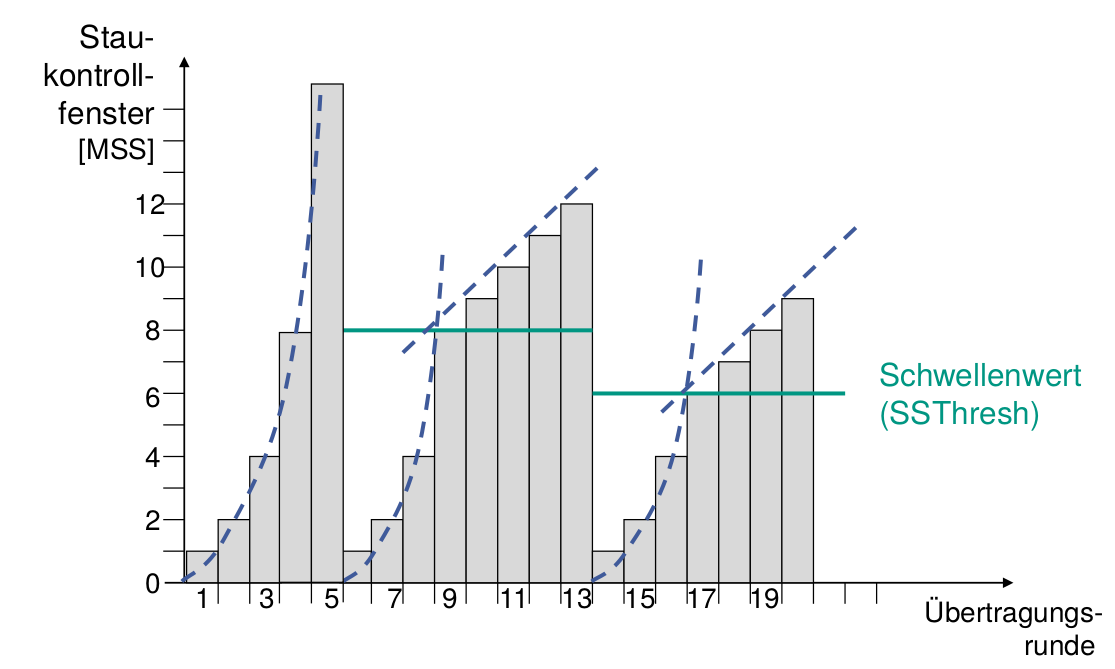
\includegraphics[width=0.33\textwidth]{TCPStaukontrolle}\end{figure}